\chapter{Other implementations\label{chap:divaonweb}}
%------------------------

In addition to the usual way of working with \diva (i.e., command line), there are other possibilities to use it without the installation of the whole code.
 
\minitoc

\newpage %  

\section{\diva-on-web}
%---------------------

The idea behind \diva-on-web is to provide the possibility for the users to perform interpolations with \diva without having to install it on their machine. The web interface suits to a single analysis with a relatively low number of data. For climatologies, which requires the repetition of numerous analysis, the use of \diva is necessary.

The server is accessible at: \url{http://gher-diva.phys.ulg.ac.be/web-vis/diva.html} and a complete description of the interface is found in \citet{BARTH10}.


\subsection{Implementation}

The web interface of \diva is based on OpenLayer (\url{http://openlayers.org/}) and is OGC-compliant (Open Geospatial Consortium, \url{http://www.opengeospatial.org/}). The server is a 2 quad-core Xeon E5420 running under Linux. The server and client software are available under GPL. The Web Map Server use \texttt{Python} language along with the plotting packages \texttt{matplotlib} (\url{http://matplotlib.org/}) and \texttt{basemap} (\url{http://matplotlib.org/basemap/}). 

\begin{figure}[htpb]
	\centering
	\parbox{.55\textwidth}{
		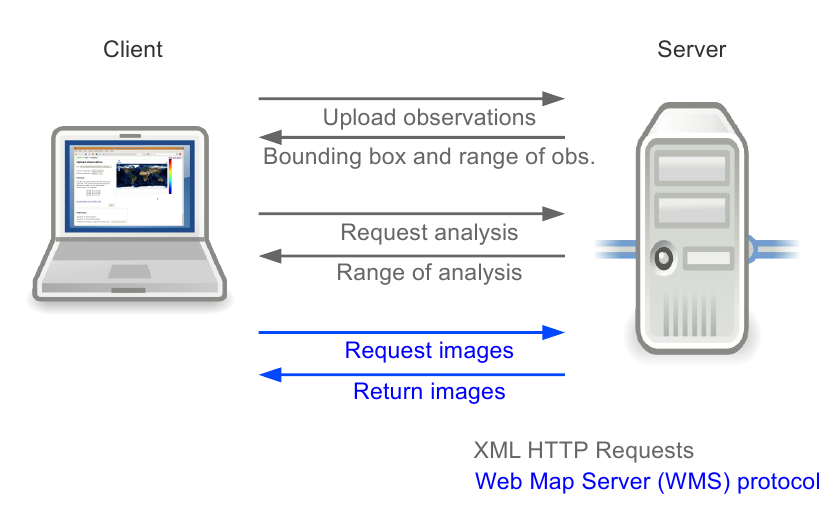
\includegraphics[width=.525\textwidth]{diva_on_web_paper1}
		}\parbox{.45\textwidth}{
		\caption{Communications between the server and the client for analysis with \diva-on-web.\label{fig:diva_on_web_paper1}}
		}
\end{figure}

\subsection{A complete example}

The steps to follow to obtain an analysed field is the following

\begin{enumerate}
\item Upload your data file (see Section~\ref{sec:dataformat} for the correct file format). \hfill (Fig.~\ref{fig:divaonweb1})
\item Define the analysis grid. \hfill (Fig.~\ref{fig:divaonweb2})
\item Select the analysis parameters. \hfill (Fig.~\ref{fig:divaonweb3})\\
The script \command{divafit} provides an estimate for the correlation length \hfill (Fig.~\ref{fig:divaonweb4})
\item Perform the analysis.\hfill (Fig.~\ref{fig:divaonweb5})
\end{enumerate}

\begin{figure}[H]
\centering 
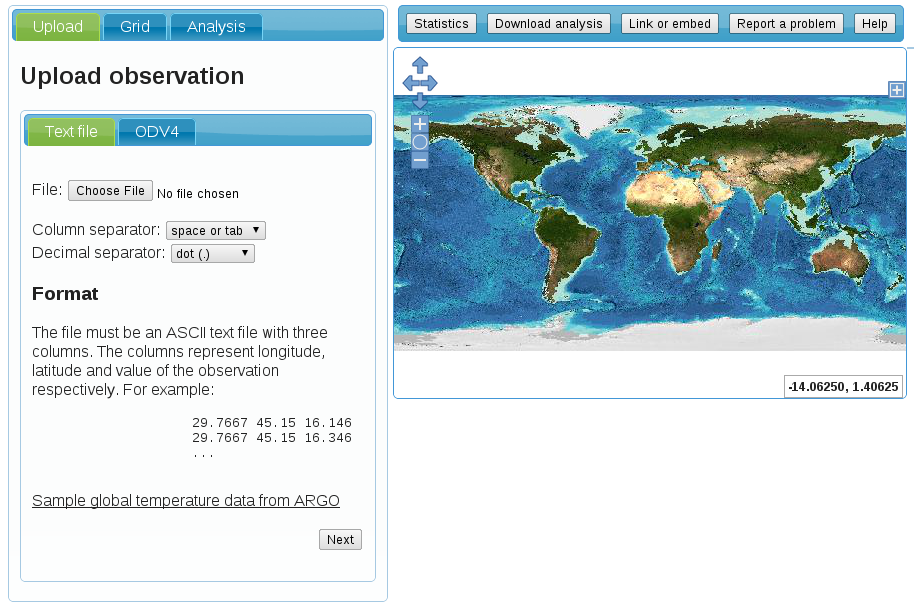
\includegraphics[width=.75\textwidth]{divaonweb1}
\caption{Upload of data.\label{fig:divaonweb1}}
\end{figure}

\begin{figure}[H]
\centering 
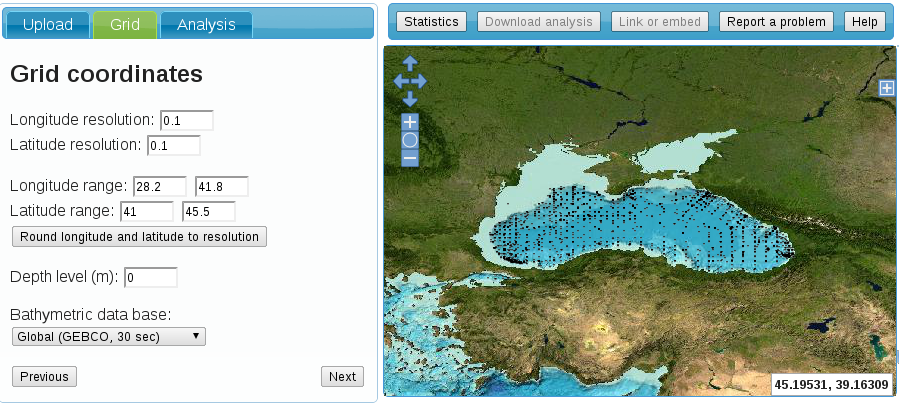
\includegraphics[width=.75\textwidth]{divaonweb2}
\caption{Grid coordinates.\label{fig:divaonweb2}}
\end{figure}

\begin{figure}[H]
\centering 
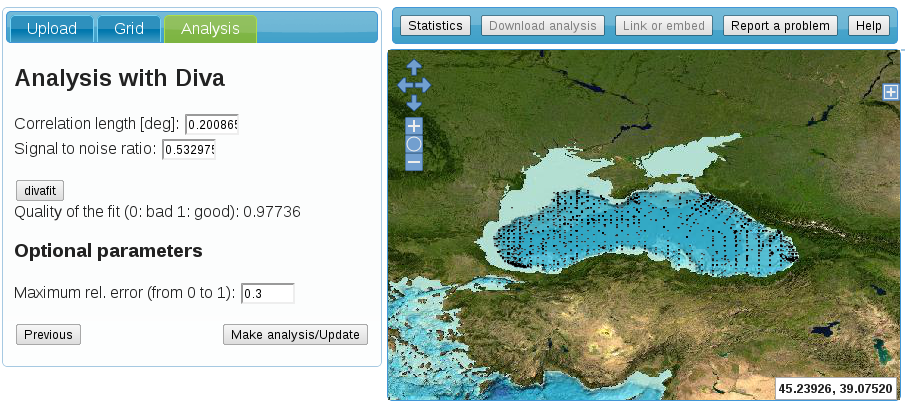
\includegraphics[width=.75\textwidth]{divaonweb3}
\caption{Parameters selection.\label{fig:divaonweb3}}
\end{figure}

\begin{figure}[H]
\centering 
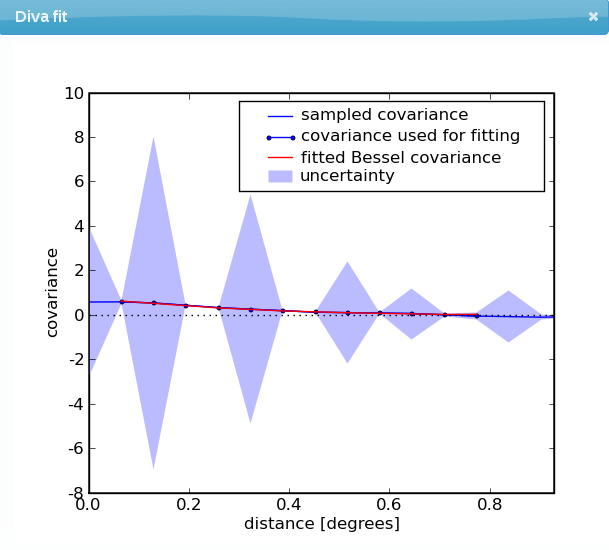
\includegraphics[width=.5\textwidth]{divaonweb4}
\caption{Visual results of \command{divafit}.\label{fig:divaonweb4}}
\end{figure}

\begin{figure}[H]
\centering 
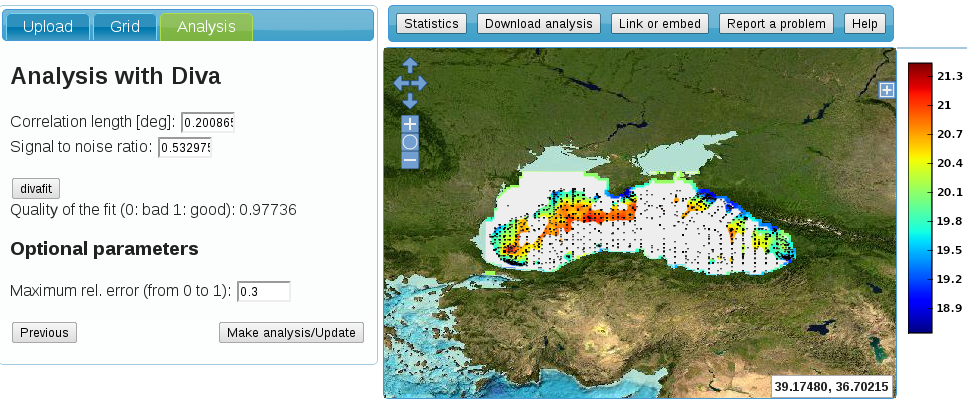
\includegraphics[width=.75\textwidth]{divaonweb5}
\caption{Analysis and mask based on relative error.\label{fig:divaonweb5}}
\end{figure}

The outputs are available in various formats (Fig.~\ref{fig:divaonweb6}): NetCDF, Matlab (or Octave) file, Keyhole Markup Language (KML) and other image formats. 

\begin{figure}[H]
\centering 
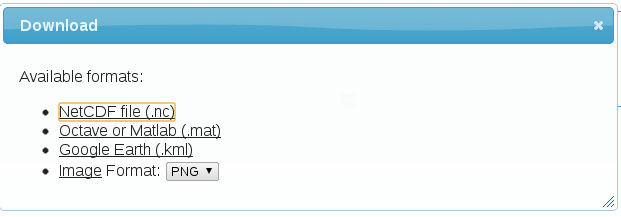
\includegraphics[width=.5\textwidth]{divaonweb6}
\caption{Exportation of the result field in different formats.\label{fig:divaonweb6}}
\end{figure}


\subsection{Conditions of use}
%-----------------------------


\begin{itemize}
\item Open to all users without registration.
\item CPU time and the number of observations is limited per user, in order to guarantee availability to all. The current maximum CPU time is 10 minutes and the maximum number of observations is 100000.
\end{itemize}


\section{Ocean Data View}
%------------------------

\index{Ocean Data View}
Ocean Data View \citep[ODV,][]{SCHLITZER02} is a tool for the analysis and visualization of oceanographic data. Among the numerous possibilities ODV, we find the production of gridded fields based on the original data. Three methods are offered \citep{SCHLITZER12}: 
\begin{enumerate}
\item \textit{Quick gridding}, a weighted averaging algorithm optimized for speed, adapted for situations with millions data points.
\item \textit{VG gridding}, a more sophisticated weighted averaging algorithm.
\item \diva gridding.
\end{enumerate}

\begin{figure}[H]
\centering 
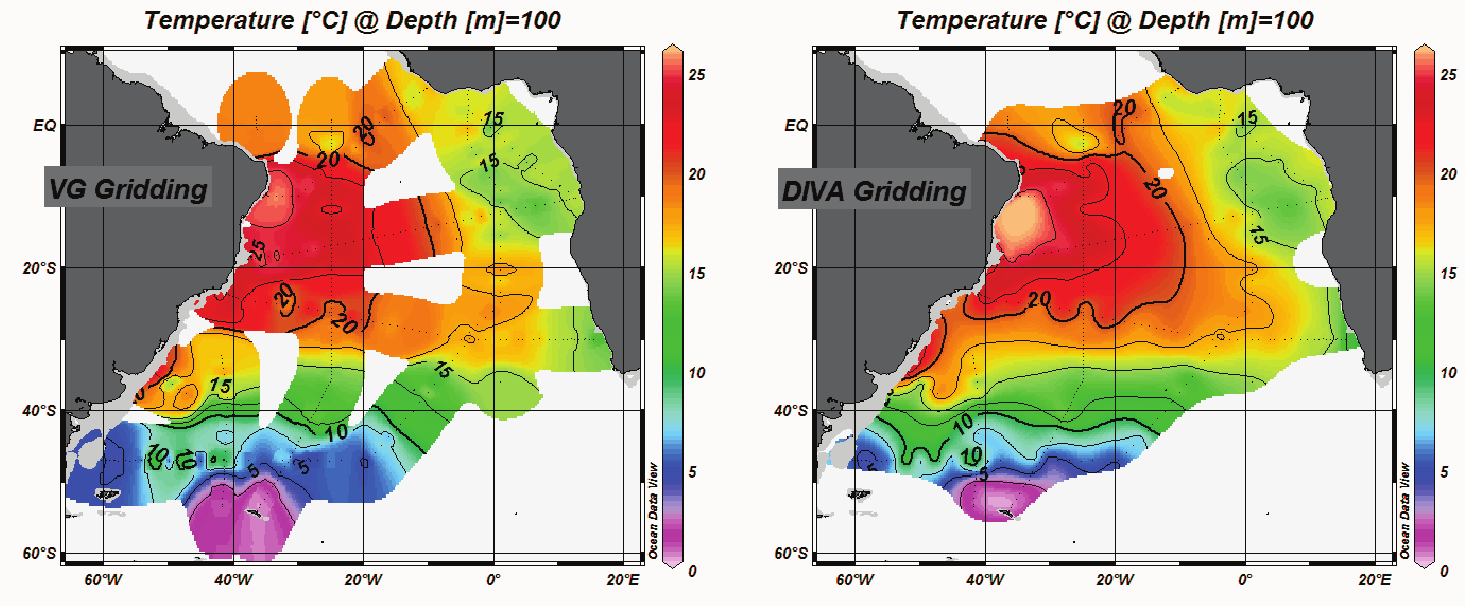
\includegraphics[width=.95\textwidth]{odvdiva1}
\caption[Example of VG gridding and \diva gridding with ODV.]{Example of VG gridding and \diva gridding with ODV (from \citet{SCHLITZER12}).\label{fig:divaodv}}
\end{figure}

\diva gridding is a simplified version of \diva implemented inside ODV, where the user can only modify a limited number of parameters.

\section{Matlab toolbox}
%------------------------

\index{Matlab}
The \diva Matlab toolbox is an interface to perform 2-D analysis without having to compile the whole code and to type commands in a terminal. 

\subsection{Installation}
%------------------------

Download the package from: \url{http://modb.oce.ulg.ac.be/mediawiki/upload/divaformatlab.zip}
and unzip the archive:
\begin{lstlisting}[style=Bash]
[charles@gher13 Software]$ wget http://modb.oce.ulg.ac.be/mediawiki/upload/divaformatlab.zip
...
[charles@gher13 Software]$ unzip divaformatlab.zip
\end{lstlisting}

The structure is the following:
\begin{lstlisting}[style=Bash]
[charles@gher13 Software]$ tree
.
|-- README
|-- divagrid.m
|-- linux_binaries
|   |-- contourgen.exe
|   |-- diva.exe
|   `-- generopt.exe
|-- testdivagrid.m
`-- windows_binaries
    |-- contourgen.exe
    |-- diva.exe
    `-- generopt.exe

2 directories, 9 files
\end{lstlisting}

The main file is \file{divagrid.m}, while \file{testdivagrid.m} provides a few example of how the function can be used.
Directories \directory{linux\_binaries} and \directory{windows\_binaries} 
 %%%%%%%%%%%%%%%% to continue here
 
\subsection{Usage}

The syntax \file{divagrid.m} is close to matlab \file{griddata.m} function, but has additional parameters.

To run \diva with matlab, \file{divagrid.m} has to be in the matlab path as well as the three executables:
\begin{itemize}
\item \texttt{contourgen.exe}
\item \texttt{generopt.exe}
\item \texttt{diva.exe}
\end{itemize}


figures (presented in diva workshop and SDN annual meeting
